\chapter{Analysis Overview}\label{sec:analysis_overview}

\section{History of the \hzg{} Search}
Both the CMS and ATLAS collaborations have undertaken the search for \hzg{} since Run 1 of the LHC. 
Before the CMS Run 2 analysis, which is the focus of this thesis, each collaboration published results using 
Run 1 data at $\sqrt s = 7$ and 8\TeV~\cite{cms-HZG,atl-HZG}, CMS published a result with 2016 data at $\sqrt s = 13\TeV$~\cite{Sirunyan:2018tbk}, and 
ATLAS published a full Run 2 result at $\sqrt s = 13\TeV$~\cite{Aad:2020plj}. As such, the present analysis represents the continuation 
of a broader effort, so we will give a brief history of these prior searches to put our work in context. While 
some of the analysis strategies of past searches inform our current strategy, there are also many differences 
and innovations in our analysis. We will emphasize the ways in which our analysis 
overlaps and differs with previous approaches, and will show that our innovations have significantly 
improved the expected sensitivity and statistical robustness of the search. 

\subsection{The Run 1 Searches}
In 2014, ATLAS published its Run 1 results~\cite{atl-HZG} for the search for \hzg{} where $\mathrm{Z}\to\ell^+\ell^-$ with $\ell=\mathrm{e}$ or $\mu$. The baseline strategy was a standard dilepton 
plus photon selection, with $m_{\ell^+\ell^-}$ near the Z boson mass and $\ell^+\ell^-\gamma$ invariant mass ($m_{\ell^{+}\ell^{-}\gamma}$) between 115 and 170\GeV. The resolution of $m_{\ell^{+}\ell^{-}\gamma}$ was improved using a kinematic fit procedure, accounting for the true Z boson line shape. Events were categorized based on lepton flavor; the pseudorapidity difference between the photon and Z boson; and the variable $p_{\mathrm{T}}^{t}$, defined as $\abs{\vec{p}_\mathrm{T}^{\,\PZ\gamma}\times\hat{t}}$, where $\hat{t}=(\vec{p}_\mathrm{T}^{\,Z}-\vec{p}_\mathrm{T}^{\,\gamma})/\abs{\vec{p}_\mathrm{T}^{\,Z}-\vec{p}_\mathrm{T}^{\,\gamma}}$~\cite{Ackerstaffetal.1998,VESTERINEN2009432}, the $\pt$ of the $\PZ\gamma$ system that is perpendicular to the difference of the three-momenta of the $\PZ$ boson and the photon, a quantity that is strongly correlated with the \pt of the $\lplm\gamma$ system. Limits on the signal strength relative to the SM prediction, shown in Fig. \ref{fig:run1_limits} (left), were obtained from a simultaneous fit to the $m_{\ell^{+}\ell^{-}\gamma}$ distributions in all categories.

The CMS Run 1 analysis~\cite{cms-HZG} was published in 2015 for the $\mpmm\gamma$ and $\epem\gamma$ final states. It employed a standard dilepton plus photon selection, but the $m_{\ell^+\ell^-\gamma}$ range was 100--190\GeV, which includes a kinematic turn-on around 110--115\GeV, mainly driven by the photon \pt selection. The choice to model this turn-on increased the complexity of the fit relative to the ATLAS analysis above, but was made in order to minimize potential bias. Events were categorized based on flavor; presence of a dijet system; lepton and photon pseudorapidity; and the photon $\mathrm{R}_9$, which is the energy sum of the 3x3 ECAL crystal array centered on the most energetic crystal divided by the supercluster energy, and is associated with the quality of the photon. The CMS Run 1 limits on the signal strength are shown in Fig. \ref{fig:run1_limits} (right). 

\begin{figure}[tb]
  \centering
   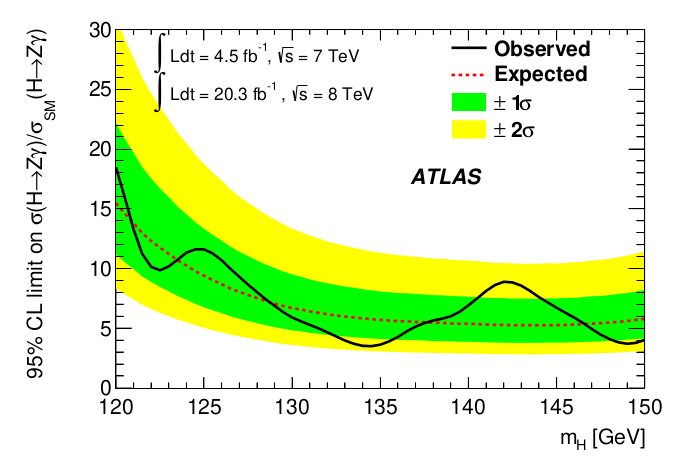
\includegraphics[width=0.45\textwidth,height=0.33\textwidth]{fig/overview/atl_run1_lim.png}
   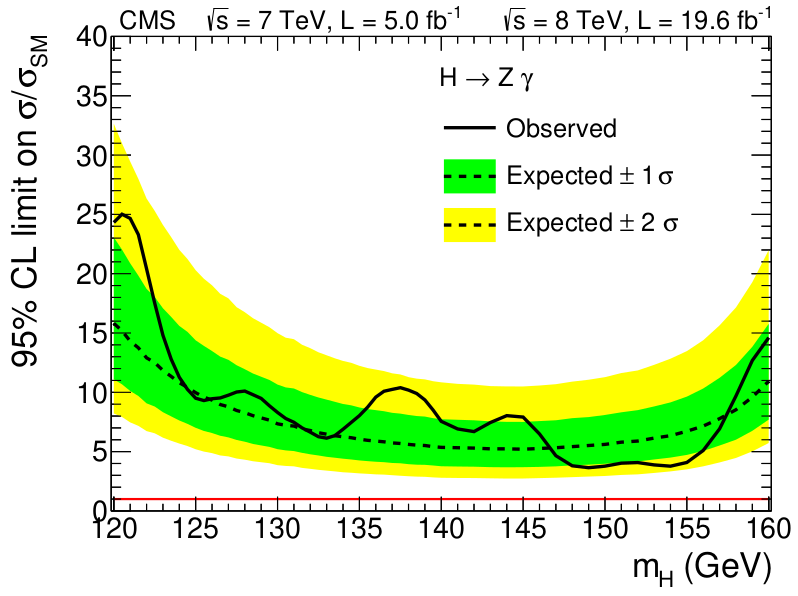
\includegraphics[width=0.45\textwidth,height=0.33\textwidth]{fig/overview/cms_run1_lim.png}
	\caption
	[ATLAS (left) and CMS (right) Run 1 limit results as a function of $m_\PH$.]
	{ATLAS (left~\cite{atl-HZG}) and CMS (right~\cite{cms-HZG}) Run 1 limit results as a function of $m_\PH$.}
	\label{fig:run1_limits}
\end{figure}


\subsection{The Previous Run 2 Searches}
The first CMS \hzg{} results at $\sqrt s = 13\TeV$~\cite{Sirunyan:2018tbk} were published in 2018 using the 2016 data set, corresponding to an integrated luminosity of 35.9\fbinv. The search strategy was largely similar to the CMS Run 1 analysis, with a few main differences. First, a boosted category was introduced to the analysis, defined by $\pt^{\lplm\gamma}>60\GeV$. This category targeted events with a Higgs boson recoiling against a jet. Second, the range of $m_{\lplm\gamma}$ was restricted to 115--170\GeV in order to avoid fitting the kinematic turn-on. The decision of whether or not to fit the turn-on became critically important in the full CMS Run 2 analysis, and will be discussed in more detail later in this thesis. Limits from the CMS 2016 search are shown in Fig. \ref{fig:run2_prev_results} (left). 

The ATLAS full Run 2 search~\cite{Aad:2020plj} was published in 2020, with a largely similar strategy to the Run 1 analysis. As in Run 1, a kinematic fit was used to improve the $m_{\lplm\gamma}$ resolution and the variable $p_{\mathrm{T}}^{t}$ was used for categorization. However, there were a few major differences introduced in the Run 2 analysis. The fit range was changed to $105\GeV < m_{\lplm\gamma} < 160\GeV$ and some aspects of the categorization strategy were updated. For categorization, the most significant change was the use of a boosted decision tree (BDT) trained to separate VBF Higgs production events from other Higgs production mechanisms and backgrounds. As will be discussed later in this thesis, the use of BDTs for categorization can significantly improve the sensitivity of searches for \hzg{}. Figure \ref{fig:run2_prev_results} (right) shows a summary of the fit results for the ATLAS Run 2 search. An excess in data was observed, corresponding to $2.2$ standard deviations for $m_{\PH}=125.09\GeV$.

\begin{figure}[tb]
  \centering
   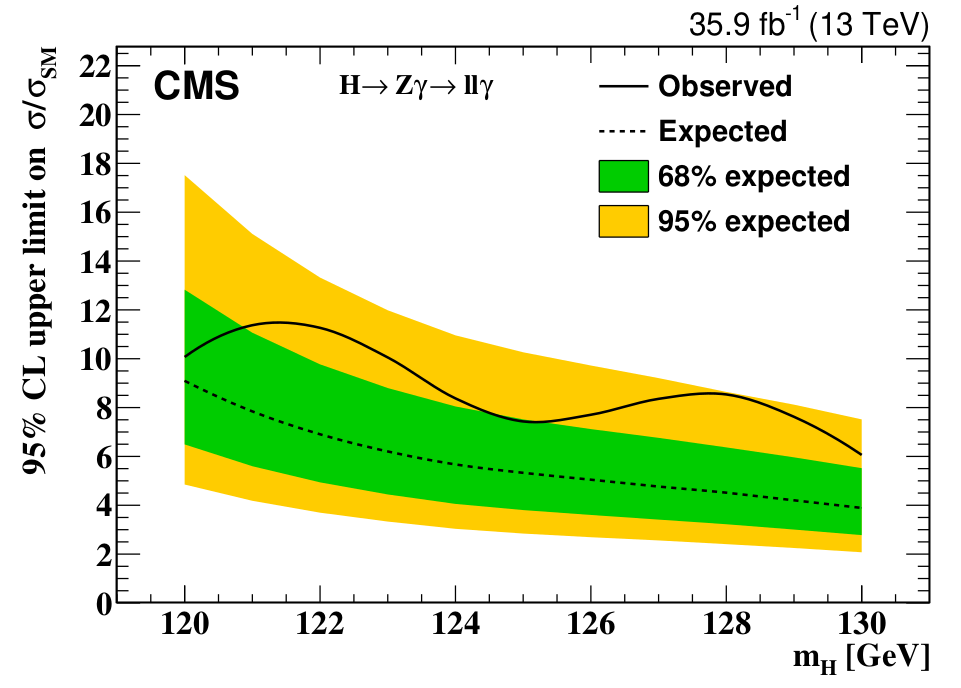
\includegraphics[width=0.45\textwidth,height=0.33\textwidth]{fig/overview/cms_2016_lim.png}
   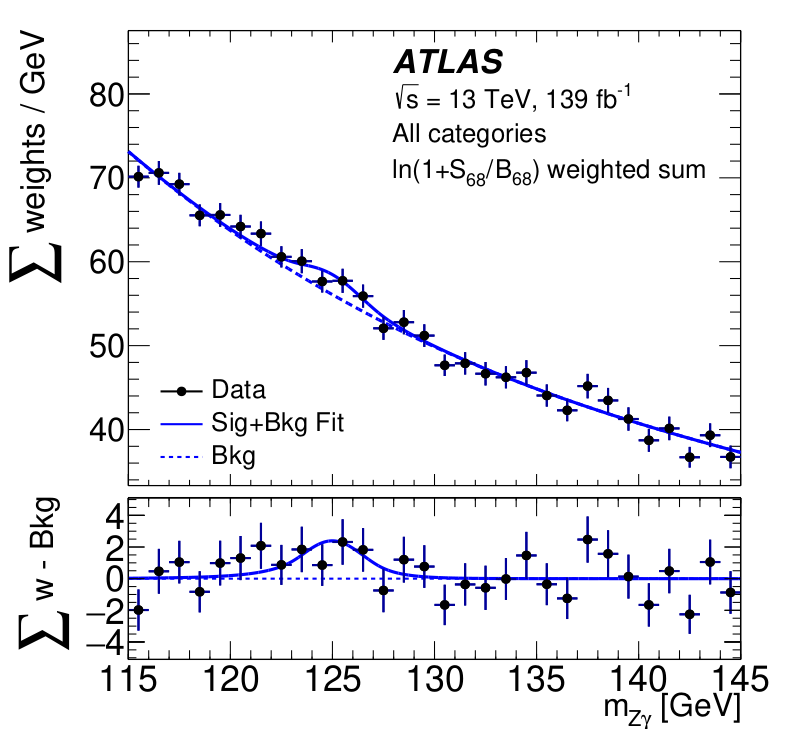
\includegraphics[width=0.45\textwidth,height=0.33\textwidth]{fig/overview/atlas_run2_fit.png}
	\caption
	[Left: CMS 2016 limit results as a function of $m_\PH$. Right: ATLAS Run 2 signal plus background fit, for $m_{\PH}=125.09\GeV$, weighted by ln(1+$\mathrm{S}_{68}/\mathrm{B}_{68})$, where $\mathrm{S}_{68}$ and $\mathrm{B}_{68}$ are the expected signal and background events in an $m_{\lplm\gamma}$ window containing 68\% of the expected signal yield.]
	{Left: CMS 2016 limit results~\cite{Sirunyan:2018tbk} as a function of $m_\PH$. Right: ATLAS Run 2 signal plus background fit~\cite{Aad:2020plj}, for $m_{\PH}=125.09\GeV$, weighted by ln(1+$\mathrm{S}_{68}/\mathrm{B}_{68})$, where $\mathrm{S}_{68}$ and $\mathrm{B}_{68}$ are the expected signal and background events in an $m_{\lplm\gamma}$ window containing 68\% of the expected signal yield.}
	\label{fig:run2_prev_results}
\end{figure}

\section{The CMS Run 2 Strategy}
The remainder of this thesis provides a thorough description of the CMS Run 2 search for \hzg{}. First, a brief overview is provided below. The data sample corresponds to an integrated luminosity of \LumiT\fbinv of $\Pp\Pp$ collisions at $\sqrt s = 13 \TeV$ accumulated between 2016 and 2018. Much of the analysis strategy has been inspired by the prior CMS and ATLAS \hzg{} searches, as well as other CMS Higgs analyses. The baseline event selection is similar to the previous CMS searches. One crucial difference with respect to the CMS 2016 analysis is that the $m_{\lplm\gamma}$ range has been extended to 105--170\GeV, including the kinematic turn-on, as was done in the CMS Run 1 analysis. This choice will be discussed in detail later in this thesis. Additionally, a kinematic fit procedure has been added to the analysis to improve the $m_{\lplm\gamma}$ resolution, similar to what has been done in the previous ATLAS \hzg{} analyses and in other CMS Higgs analyses, including $\PH\to\PZ\PZ^*\to4\ell$~\cite{bib:htozz2016}.

The sensitivity of the analysis is enhanced by searching for Higgs boson production in a variety of mechanisms, including gluon-gluon fusion ($\Pg\Pg\PH$); vector boson fusion (VBF); and the associated production of a Higgs boson with either a weak vector boson (V$\PH$, where V = $\PZ$ or $\PW$) or a top quark pair ($\ttbar\PH$). The dominant backgrounds arise from Drell--Yan production in association with an initial-state photon~($\PZ/\gamma^{*}$+$\gamma$) and Drell--Yan production in association with jets, where a jet or additional lepton is misidentified as a photon ($\PZ/\gamma^{*}$+jets). 
After using a set of discriminating variables to suppress background in the different production mechanisms, the signal is identified as a narrow resonant peak around $m_{\PH}$ in the distribution of $m_{\lplm\gamma}$.

The data sample is divided into mutually exclusive categories according to (i) the presence of an additional lepton produced by $\PZ(\to\lplm)$ or $\PW(\to\ell\nu)$ decay, indicating the possible associated production of a Higgs boson with a $\PW$ or $\PZ$ boson, or $\ttbar\PH$ production with a leptonic top quark decay; (ii) the value of a multivariate analysis (MVA) discriminant characterizing the kinematic properties of a dijet system together with the $\lplm\gamma$ candidate, indicating possible VBF production; and (iii) the value of an MVA discriminant characterizing the kinematic properties of the $\lplm\gamma$ system. This MVA categorization procedure is an innovation of the CMS Run 2 analysis. While a VBF MVA was used in the ATLAS full Run 2 analysis, we are the first to also leverage a kinematic MVA for maximal discrimination between signal and background.
